\section{Introduction to the Ising Model}
We have now done a quick (and likely wholly inadequate) review of basic statistical mechanics. From here, we will begin to study phase transitions. We will study on a simple type of phase transition (with some side comments about others) - this is because there is a lot to be learned just by considering this simple example of magnetic/Ising systems. Most of the action here happened in the 1980s (so we aren't learning anything extremely new here) but this is just how physics classes go (but we will discuss the conformal bootstrap at the end of the course, which is something invented this century).

The Ising model was initially studied and solved in one dimension, where there are no phase transitions; it was then initially erroneously concluded that there are no phase transitions in any dimension. Later on it was solved exactly in two dimensions, where it was shown that there was a second order phase transition. This then became the standard model system to consider in the study of phase transitions. Through our study of this system, there is a huge amount of theoretical physics that are seeded by it (e.g. QFT). Even more than that, the language of these fields has largely inspired by the Ising model.

\subsection{The Hamiltonian}
We will use the canonical ensemble to study the Ising model. This is a physical model, so there is a Hamiltonian $H$ which describes the energy of a configuration, and a density:
\begin{equation}
    \rho = \frac{e^{-H/k_B T}}{Z}
\end{equation} 
with $Z$ the partition function:
\begin{equation}
    Z = \sum_{\text{states}}e^{-H/k_B T}.
\end{equation}
We have the thermodynamic quantity of the Helmholtz free energy:
\begin{equation}
    F = -k_B T \ln Z.
\end{equation}
These are the very general statistical mechanical ingredients. Let's talk about the model itself. It is a model of a magnetic system in one dimension, composed of a number of spins arranged on a lattice. If the spins like to align with each other, then we have a ferromagnetic material, if the spins like to anti-align per-site then we have a antiferromagnet.

How do we describe these spins? We can describe a spin at point $x$ by:
\begin{equation}
    \sigma_x = \begin{cases}
        +1 \\ -1
    \end{cases}
\end{equation}
i.e. a spin at position $x$ which either points up or down. $x$ lives on a lattice; a 2-D lattice is sketched as an example below:

\begin{figure}[htbp]
    \centering
    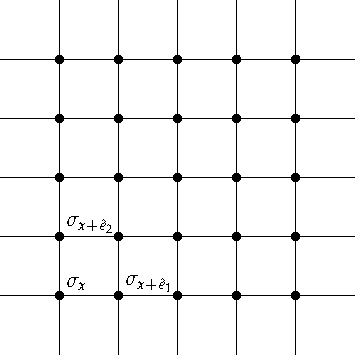
\includegraphics[]{Images/fig-2DIsing.pdf}
    
    \caption{2D Ising model on a square lattice. The spins sit on the nodes/crossings of the lattice, with interaction between neighbouring spins ($\mu = \pm \hat{e}_1, \pm \hat{e}_2$).}
    \label{fig-2DIsing}
\end{figure}

Typically we work in the thermodynamic limit where the lattice is very large (in this limit the boundary conditions should not be important to understand the physics, but this is something we can check). Writing down the Hamiltonian, we have:
\begin{equation}
    H_{interaction} = -J \sum_{x, \mu}\sigma_{x}\sigma_{x+\mu}
\end{equation}
Where $\mu$ runs over the vectors that point to the nearest neighbours of $x$ (so $x + \mu$ runs over the nearest neighbours of $x$). We will not concern ourselves too much with the lattice constant (we can just set it to one). Note that $\sigma_x\sigma_{x+\mu}$ is minimized if the two spins align, (as then $\sigma_x\sigma_{x+\mu}$ is positive and hence the negative sign out front gives the term a negative contribution). We can change the nearest neighbours assumption to include next nearest neighbours, infinite range etc. (and we can also change the behaviour of the interactions) but realistic interactions are short range so for now nearest neighbours is good to consider.

This is almost the Ising model; we can also add a coupling term to an external magnetic field:
\begin{equation}
    H_{B} = -B\sum_x \sigma_x
\end{equation}
where the spins will want to align with $B$ so as to lower the energy. So the Ising Hamiltonian is:
\begin{equation}
    H = H_{interaction} + H_{B} = -J \sum_{x, \mu}\sigma_{x}\sigma_{x+\mu} - B\sum_x \sigma_x.
\end{equation}
This simple two-parameter ($J, B$) model is already quite interesting. From it we will learn about universality - phase transitions tend to be the same for a large number of microsystems, e.g. the critical behavior for the Ising model and for liquid gas phase transition is the same. So this is why we can get away with studying something so simple.

\subsection{Analyzing the Ising Model - Phase Diagram Boundaries}
What we would like to compute is the partition function:
\begin{equation}
    Z = \sum_{\text{spins}}e^{-H/k_B T}
\end{equation}
and we would then like to calculate the free energy $F$, which is a function of the temperature $T$, the field $B$, and the number $N$:
\begin{equation}
F[T, B, N] = -k_B T \ln Z
\end{equation}
if we can find $F$, we can get all sorts of physical quantities, e.g. magnetization, susceptibility etc. For example we have the magnetization (average sum over all spins):
\begin{equation}\label{eq-magnetization}
    M = \left.-\dpd{F}{B}\right|_{N, T} = \frac{\sum_{\text{spins}}(\sum_x \sigma_x)e^{-H/k_B T}}{Z}
\end{equation}

As mentioned previously, we will assume that $N \to \infty$ (thermodynamic limit). What is left in our free energy is $T$ and $B$. So, we can draw a phase diagram:

\begin{figure}[htbp]
    \centering
    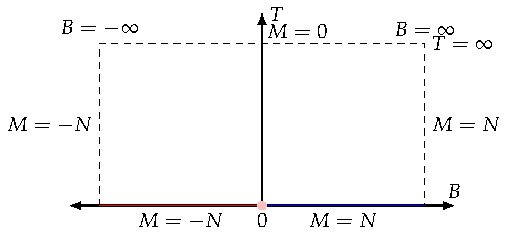
\includegraphics{Images/fig-Isingphasediagramboundaries.pdf}
    
    \caption{Phase Diagram Boundaries for the Ising Model, plotting temperature $T$ and magnetization $M$. As $B = \pm \infty$, the spins want to align all upwards ($M = N$)/downwards ($M = -N$) respectively. As $T \to \infty$, all configurations are equally likely and so $M = 0$. At $T = 0$, all spins aligning minimizes the energy and so for $B < 0$ we have $M = -N$ and for $B > 0$ we have $M = N$. At $T = 0, B = 0$ there is a first order phase transition.}
    \label{fig-Isingphasediagramboundaries}
\end{figure}

Note that as $T \to \infty$, we would first notice that our lab had burned down, but before that we would also notice that our material is no longer a ferromagnetic; it is a paramagnet with $M = 0$. We can see this from our expression for $M$ in Eq. \eqref{eq-magnetization}, where if $T \to \infty$ then $e^{-H/k_B T} = 1$ and so the up and down spins have equal weight, so the net summation comes out to zero.

At $B = \pm \infty$, we have $M \neq 0$. Specifically, if $M = \infty$ then all the spins want to align upwards so $M = N$ and if $M = -\infty$ then the spins want to align downwards so $M = -N$. As the temperature goes to zero, we are interested in the lowest energy state of the Hamiltonian. As all the spins are aligned, this minimizes the energy so actually we find $M = -N$ for all $B < 0, T = 0$ and $M = N$ for all $B > 0, T = 0$. What happens then at $B = 0$? We have a phase transitions between the two domains. We have a first order phase transition there where the magnetization completely flips.

What does the order of the phase transition mean? It refers to the number of the derivatives we can take of the free energy before the derivative does not exist. Here (at $T = 0$), $M = \text{sign}(B) N$, and the derivative of this does not exist at $B = 0$; so the first derivative of $F$ exists but the second one does not, so it is a first order phase transition. This comes from the Landau classification of phase transitions. This is not the full story; we have discovered many topological phases in recent times, and it could be argued that the classification of phases is not yet complete. If we integrate, at $T = 0$ we find $F = J\abs{B}$; this is continuous but not differentiable so the phase transition is first order.

\begin{figure}[htbp]
    \centering
    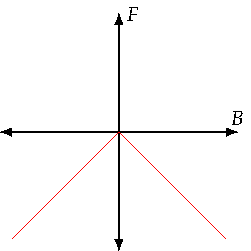
\includegraphics{Images/fig-FT0Ising.pdf}
    
    \caption{Plot of $F$ at $T = 0$ as a function of $B$. The free energy is continuous but not differentiable, and hence there is a first-order phase transition at $B = 0$. The slope of the free energy is $-J/J$.}
    \label{fig-FT0Ising}
\end{figure}

\subsection{Analyzing the Ising Model - $B = 0$ and Spontaneous Symmetry Breaking}
The line of $B = 0$ is interest. This is because the Hamiltonian has more symmetry in this case; namely the symmetry of flipping every $\sigma_x \leftrightarrow -\sigma_x$, or a $\mathbb{Z}_2$ symmetry (which can be represented, e.g. as $\set{1, -1}$ with multiplication). The magnetic field breaks this symmetry.

Note that if we are at some point in the right half of the phase diagram and we do a $\mathbb{Z}_2$ transformation, we map to the point on the other (left) side of the phase diagram (so on the $B = 0$ axis, we do not move at all!) Note however we cannot use symmetry to conclude that $M = 0$ at $B, T = 0$; as the magnetic moment here is dependent on the prior history of the system (how was this critical point reached). So we have some strange behaviour here; at this point, the Hamiltonian has $\mathbb{Z}_2$ symmetry but the actual state of the system does not inherit this symmetry; the system chooses one of the totally magnetized states depending on the prior history. This is known as \emph{spontaneous symmetry breaking}.

Now we can ask; if we go up the $B = 0$ axis (by turning on the temperature) from the $B, T = 0$ point, what happens? Does the symmetry remain broken? In the 1-D Ising model, there is a phase transition where the symmetry is unbroken; the magnetization goes back to $M = 0$. We will show that this comes about through solving the model. In higher dimensions, we cannot exclude the possibility that $M \neq 0$ persists for a while even as we turn up $T$; for example it might be possible that $M$ decays up to some point after hitting zero. We then have a discontinuity in the phase diagram partially along the $T = 0$ axis. We have a line of first order phase transitions, and it ends at some point in a second order phase transition. Unlike the boundaries of the diagrams, we have not really justified this statement; we will have to return to its proof later. 

\begin{figure}[htbp]
    \centering
    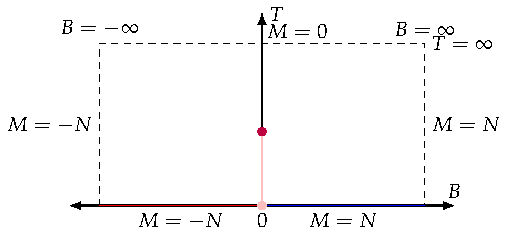
\includegraphics{Images/fig-IsingphasediagramB0.pdf}
    \caption{For dimensions larger than 1, $M \neq 0$ persists at $B = 0$ even as the temperature is tuned up. This results in a ``first order phase transition line'' partway up the $B = 0$ axis, culminating in a second order phase transition point.}
    \label{fig-IsingphasediagramB0}
\end{figure}

It is difficult to study the phase transitions in generality, so we will (later) focus our attention to the point around the second order phase transition. Specifically, things are complicated by the magnetic field, so we will study a neighbourhood of the second order phase transition that lies on the $B = 0$ axis.

We will be able to study the 1-D model in full generality, but this is not very interesting as the ``phase transition line'' we see above will get shrunk to a point. The 2-D model has been solved but only at $B = 0$. 

\subsection{Solving the 1-D model}
One of the slightly unsatisfying things about the study of this system is that the models in different dimensions have different ad-hoc ways of solving them analytically. When we start to look at approximations, we will see a unifying formalism (e.g. renormalization group).

We consider the 1-D Ising model, which is just a chain of classical spins. 

\begin{figure}[htbp]
    \centering
    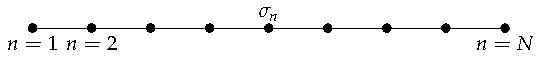
\includegraphics{Images/fig-1DIsing.pdf}
    \caption{Cartoon of 1D Ising model (pictured with $N = 9$ spins). The spin at site $n$ is denoted $\sigma_n$.}
    \label{fig-1DIsing}
\end{figure}

The Hamiltonian takes the form:
\begin{equation}
    H = -H\sum_{n=1}^{N-1}\sigma_n \sigma_{n+1} - B\sum_n \sigma_n
\end{equation}
The route to the solution here is just a brute-force calculation of the partition function:
\begin{equation}
    Z = \sum_{\sigma_1 = \pm 1, \ldots, \sigma_n = \pm 1} e^{\frac{J}{k_B T}\sum_n \sigma_n \sigma_{n+1} - \frac{B}{k_B T}\sum_{n}\sigma_n}
\end{equation}
we rewrite this as an extended multiplication:
\begin{equation}
    Z = \sum_{\sigma_1 = \pm 1} \sum_{\sigma_2 = \pm 1} \ldots \sum_{\sigma_n = \pm 1}e^{-\frac{B}{2k_B T}\sigma_1}\left[e^{\frac{J}{k_B T}\sigma_1 \sigma_2 - \frac{B}{2k_B T}(\sigma_1 + \sigma_2)}\right]\left[e^{\frac{J}{k_B T}\sigma_2 \sigma_3 - \frac{B}{2k_B T}(\sigma_2 + \sigma_3)}\right] \ldots \left[e^{\frac{J}{k_B T}\sigma_{N-1} \sigma_N - \frac{B}{2k_B T}(\sigma_{N-1} + \sigma_N)}\right]e^{-\frac{\beta}{2k_B T}\sigma_N}
\end{equation}
Why would we do this? Because we can take the objects inside the square brackets and call it a 2x2 matrix $T_{ab}$ (with elements that depend on whether the spins are up or down):
\begin{equation}
    T_{ab} = e^{\frac{J}{k_B T}\sigma_a \sigma_b - \frac{B}{2k_B T}(\sigma_a + \sigma_b)}
\end{equation}
where $T_{11}$ has $\sigma_a = \sigma_b = 1$, $T_{22}$ has $\sigma_a = \sigma_b = -1$ and so on. Explicitly:
\begin{equation}
    T_{ab} = \m{e^{\frac{J-B}{k_B T}} & e^{-\frac{J}{k_B T}} \\ e^{-\frac{J}{k_B T}} & e^{\frac{J + B}{k_B T}}}
\end{equation}
We can then write the partition function as:
\begin{equation}
    Z = \sum_{\sigma_1 = \pm 1}\sum{\sigma_N = \pm 1} e^{-\frac{B}{2k_B T}\sigma_1}(T^{N-1})_{\sigma_1\sigma_N} e^{-\frac{B}{2k_B T}\sigma_N}
\end{equation}
what does this buy us? Because $T_{ab}$ is real and symmetric, it can be diagonalized by a similarity transform. So, $T$ can be written as:
\begin{equation}
    T = R\Lambda R^T = \m{\cos\theta & -\sin\theta \\ \sin\theta & \cos\theta}\m{t_+ & 0 \\ 0 & t_-}\m{\cos\theta & \sin\theta \\ -\sin\theta & \cos\theta}
\end{equation}
with $R$ rotation matrices. The partition function then becomes:
\begin{equation}
    Z = \sum_{\sigma_1 = \pm 1, \sigma_N = \pm 1} e^{-\frac{B}{2k_B T}\sigma_1}R\m{t_+^{N-1} & 0 \\ 0 & t_-^{N-1}}R^T e^{-\frac{B}{2k_B T}\sigma_N}
\end{equation}
where we have used that $RR^T = R^TR = \mathbb{I}$ and so all but the first and last rotation matrices cancel. 

Now, what happens here? Since $N$ we take to be large, one of the eigenvalues will grow much more and will dominate. If we are interested in taking a logarithm of $Z$ and choosing the part that grows like $N$, we can just look at the larger eigenvalue. We don't really have to calculate the details if we just figure out what the larger of the two eigenvalues of the transfer matrix is; we can just consider:
\begin{equation}
    F = -k_B T N \ln t_+.
\end{equation}
But we are out of time, so we leave this to next class...
